%************************************************
\chapter{Design considerations}\label{ch:design} % $\mathbb{ZNR}$
%************************************************

This chapter should provide a very general overview over the developed system, mainly describing the employed architecture.

\section{Architectural overview}
\label{sec:architectural overview}

The application was developed taking into account the principle of separating the program logic from interface design. To support this approach the \acf{MVP} design pattern was utilised.

In this pattern the presenter separates the \ac{GUI} from the logical part of the application. The view communicates with the model only through the presenter. However, the model can notify the view directly of  data-changes if an observer-pattern or data-binding is employed\footnote{More information can be found at \textcite{Boodhoo2006}.}:

\begin{figure}[H]
\begin{center}
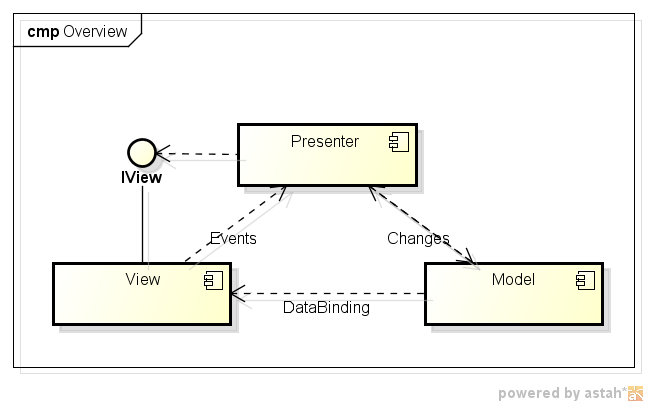
\includegraphics[width=\textwidth]{gfx/architecture_overview.png}
\caption{Architecture overview with \ac{MVP}}
\label{fig:architecture_overview}
\end{center}
\end{figure}

Noteworthy is the \texttt{IView}-interface that allows the presenter to collect all needed data from the \ac{GUI} without knowing what kind of \ac{GUI} was used. This can help in reusing the presenter for multiple application-front-ends like WinForms or ASP.NET.

In the implementation part changes that occur in the model, will be forwarded to the view via the data-binding mechanisms provided by WinForms.
% TODO put reference.

The implementation of this pattern splits the application into two projects:
\begin{description}
\item[UserInterface:] Hosts the graphical user interface and all code related to changing the appearance of the application.
\item[ApplicationLogic:] Hosts the \texttt{presenter} and the \texttt{model} component of the diagram.
\end{description}

Certain decisions made concerning these two packages will be described now, whereas greater detail will be put on implementation detail in \autoref{ch:developer_guide}.

\section{User Interface}
\label{sec:user_interface}

The \ac{GUI} was developed completely in WinForms utilizing only standard controls provided by the .NET framework.

To always display accurate data from the model, data-binding was used to connect the view to the model (further information about the concrete implementation can be found in \autoref{sec:design_user_interface}).

The \ac{GUI} project itself handles all changes to the \ac{GUI}-elements (color changes, displaying new windows, etc.), whereas the collection of input-data from the controls is performed in the presenter via interfaces (more information  in \autoref{sec:design_user_interface}).

\section{Application Logic}
\label{sec:application_logic}

\begin{figure}[H]
\begin{center}
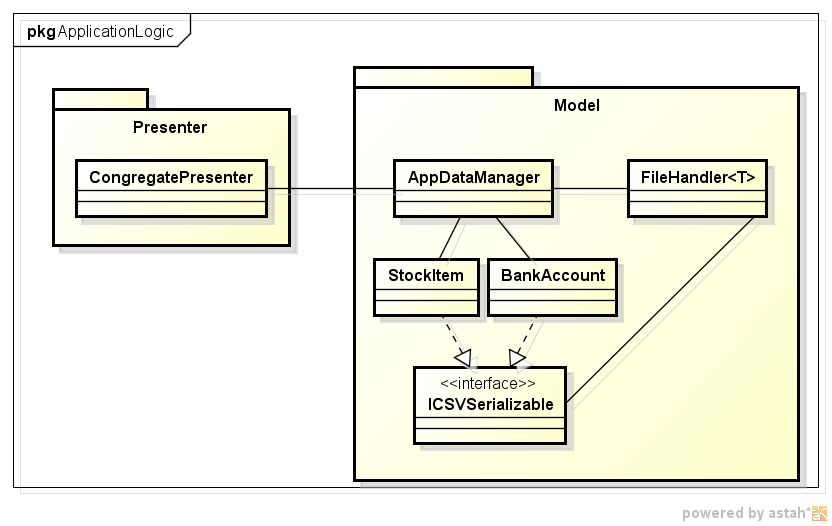
\includegraphics[width=\textwidth]{gfx/application_logic.png}
\caption{Abstract overview of project \texttt{application logic}}
\label{fig:application_logic}
\end{center}
\end{figure}

The application logic project was implemented in a very straight forward manner:

There is one class that handles all incoming requests - the \textit{AppDataManager}. 
It coordinates statements as needed: e.g. check if enough money is present on bank account $\rightarrow$ place order $\rightarrow$ update stock item.
Moreover the lists holding the stock items and bank accounts are managed by this class.

Naturally the classes for handling bank accounts and stock items are implemented in the application-logic-project as well. Moreover, a generic file handler (see \autoref{subsec:filehandler} for implementation details) and an error-handling-facility (see \autoref{subsec:error_handling}) were implemented.

Noteworthy is the fact that \texttt{BindingList}s were used in the \texttt{AppDataManager} to store the bank account and stock item lists. This was necessary to allow the data-binding with the view to work.

The \texttt{CongregatePresenter} seen in the picture is the connection point for the \ac{GUI} part of the application and mostly forwards the requests to the \texttt{AppDataManager}.